\documentclass[11pt,a4paper]{article}
\usepackage[T1]{fontenc}
\usepackage{mathptmx}
\usepackage{courier}
\usepackage[a4paper,margin=2.2cm]{geometry}
\usepackage{float,needspace,graphicx,booktabs,amsmath,xcolor,titlesec,caption,enumitem,microtype}
\usepackage[hidelinks]{hyperref}
\definecolor{navy}{HTML}{14305C}
\definecolor{gold}{HTML}{C8981E}
\titleformat{\section}{\needspace{5\baselineskip}\large\bfseries\color{navy}}{\thesection.}{0.5em}{}[{\color{gold}\titlerule[0.6pt]}]
\titleformat{\subsection}{\normalsize\bfseries\color{navy}}{\thesubsection}{0.5em}{}
\titlespacing*{\section}{0pt}{10pt}{5pt}
\titlespacing*{\subsection}{0pt}{7pt}{2pt}
\captionsetup{font=small,labelfont={bf,color=navy}}
\setlength{\parindent}{0pt}\setlength{\parskip}{4pt}
\renewcommand{\baselinestretch}{1.02}
\setlength{\textfloatsep}{8pt}\setlength{\intextsep}{7pt}
\graphicspath{{../results/figures/}}
\newcommand{\NWords}{472}
\newcommand{\NFiles}{59}
\newcommand{\NYes}{249}
\newcommand{\NNo}{223}
\newcommand{\TimeBase}{81.9}
\newcommand{\Major}{52.7}
\newcommand{\LenYes}{0.37}
\newcommand{\LenNo}{0.39}
\newcommand{\PCAone}{22}
\newcommand{\TestYes}{59}
\newcommand{\TrainYes}{46}
\newcommand{\LRcleanZero}{69.1}
\newcommand{\SVMcleanZero}{54.7}
\newcommand{\MLPcleanZero}{54.1}
\newcommand{\MLPmultiZero}{94.9}
\newcommand{\SVMmultiZero}{92.8}
\newcommand{\SVMmultiMinus}{80.3}
\newcommand{\MLPmultiMinus}{80.1}
\newcommand{\NBmultiZero}{55.7}
\newcommand{\KNNmultiZero}{74.2}
\newcommand{\SVMlcOne}{62.7}
\newcommand{\SVMlcThree}{90.9}
\newcommand{\SVMlcFive}{99.7}
\newcommand{\KNNlcOne}{96.3}
\newcommand{\MLPlcOne}{94.8}


\begin{document}
\begin{center}
{\color{navy}\rule{\textwidth}{1.2pt}}\\[6pt]
{\LARGE\bfseries\color{navy} Audio Classification: Yes/No Words}\\[4pt]
{\large Mini Task 8 Report, Digital Speech Processing}\\[6pt]
Natiq Hassan Al Abboody \quad|\quad Student ID: 404131065\\
Instructor: Dr. Mohammad Khalooei \quad|\quad November 2026\\[2pt]
{\color{gold}\rule{\textwidth}{0.8pt}}
\end{center}

\section{Introduction}
In this mini task we were asked to take an audio data set, look at its signals, sample rate and labels, and compare at least four classifiers, including an SVM and a neural network. I worked with the Yes/No corpus from the Kaldi project, which is also the data set used in the instructor's Kaldi tutorial~\cite{khalooei}, and I tried six classifiers.

My first results were close to 100\% for every model, which left me with no real comparison to report. I therefore added two experiments: testing the models on words with added white noise, and training them on very few recordings. Most of the differences discussed in this report come from these two experiments.

\section{The data set}
The corpus~\cite{openslr} contains 60 mono recordings at 8~kHz with 16-bit samples, so the signal only covers 0--4~kHz. One male speaker says eight words in each file, and each word is ``yes'' or ``no'' in Hebrew (\emph{ken} and \emph{lo}). There is no separate transcript, because the labels are written in the file name: \texttt{0\_1\_1\_0\_0\_1\_1\_0.wav} means no, yes, yes, no, no, yes, yes, no. Recordings last between about 5 and 7~seconds. OpenSLR and the instructor's tutorial say the language is Hebrew, while the README in the GitHub copy I downloaded says English. I followed OpenSLR. This makes no difference to the experiments, since the models only see the two word classes.

Figure~\ref{fig:rec} shows one recording. The words are easy to see in the waveform, with quiet gaps between them. The spectrogram also has faint horizontal lines at fixed frequencies between the words as well as during them. Speech would not behave like that, so they are probably a steady hum picked up during recording.

\begin{figure}[H]\centering
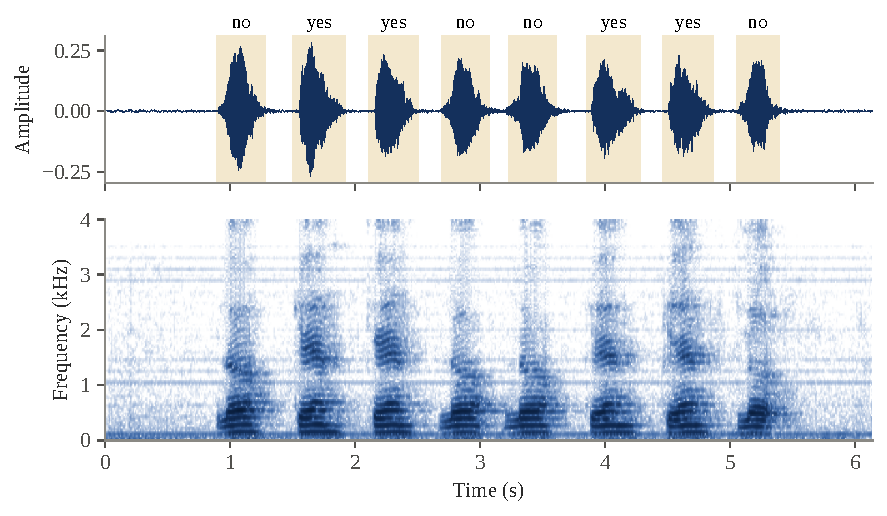
\includegraphics[width=0.86\textwidth]{fig1_recording.pdf}
\caption{Waveform and spectrogram of \texttt{0\_1\_1\_0\_0\_1\_1\_0.wav}. The shaded regions are the automatically detected words, with labels taken from the file name.}\label{fig:rec}
\end{figure}

\section{Method}
\subsection{Cutting recordings into words}
Each file has eight labels, so it has to be cut into eight words before any word can be classified. I computed the short-time log energy, smoothed it, and tried many thresholds between the noise floor and the peak. Several thresholds usually give exactly eight regions. I took the middle one, because a threshold at the top of that range can cut off the weak end of a word. Each region was then extended by 50~ms on both sides.

This gave eight words in 59 files. The exception was \texttt{0\_1\_0\_1\_0\_0\_0\_0.wav}. After the seventh word its energy stays at the noise floor until the end of the file, so it seems to contain only seven audible words although its name lists eight. I could not tell which label was missing, so I left this file out. The final set has \NWords{} words from \NFiles{} recordings: \NYes{} yes and \NNo{} no. I did not check the segments by listening to all of them. The near-perfect results below do suggest that words and labels are correctly aligned, since a shifted label would appear as a classification error.

\subsection{Features}
Figure~\ref{fig:yn} compares one ``yes'' with one ``no''. Their energy is distributed differently over frequency, which gives a first sign that spectral features should work well. I used MFCCs~\cite{davis}, which I wrote with NumPy and SciPy so that each step stayed visible: pre-emphasis with $\alpha=0.97$, 25~ms Hamming frames with a 10~ms hop, a 256-point FFT, 26 mel filters and 13 cepstral coefficients. The delta coefficients are regression slopes over $\pm 2$ frames:
\begin{equation}
d_t=\frac{\sum_{i=1}^{2} i\,(c_{t+i}-c_{t-i})}{2\sum_{i=1}^{2} i^2}.
\end{equation}
The mel step is a filter bank, meaning a set of band-pass filters that splits a signal into sub-bands~\cite{filterbank}. Windowed FFTs on overlapping frames already act as a bank of narrow filters, and the 26 triangular mel filters then group these FFT bins into wider bands. I only need this analysis side of a filter bank, because nothing has to be reconstructed. The DCT then turns the 26 log energies into cepstral coefficients.

Words have different lengths, but the classifiers need an input of fixed size. For each of the 39 coefficient tracks I therefore took the mean and standard deviation over the word, which gives 78 values. I removed the mean of $c_0$ in each word to reduce the effect of loudness, so that one of the 78 values is always zero. For comparison, I also trained an SVM on three simple time-domain values: duration, mean zero-crossing rate and RMS level.

\begin{figure}[H]\centering
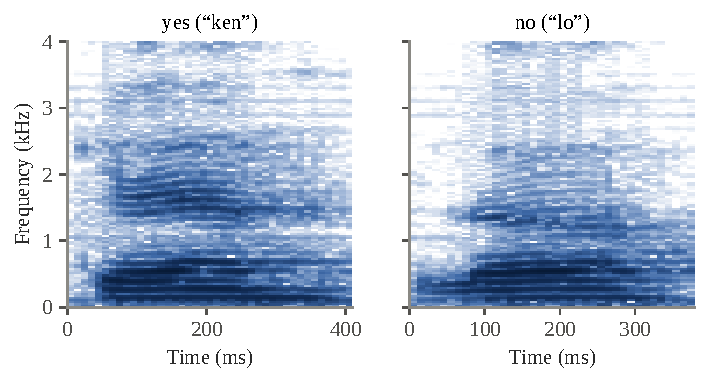
\includegraphics[width=0.62\textwidth]{fig2_yes_no.pdf}
\caption{Spectrograms of one ``yes'' and one ``no'' from the recording in Figure~\ref{fig:rec}.}\label{fig:yn}
\end{figure}

\subsection{Classifiers and evaluation}
All models come from scikit-learn~\cite{sklearn}. Features were standardised with values computed on the training data, except for the random forest, which does not need this. The tested settings were:
\begin{itemize}[nosep,leftmargin=*]
\item \textbf{SVM}~\cite{cortes} with an RBF kernel: $C\in\{1,10,100\}$, $\gamma\in\{\text{scale},0.001\}$.
\item \textbf{Neural network}: an MLP with hidden layers of (32) or (64, 32) units, and $L_2$ penalty $\alpha\in\{10^{-4},10^{-2}\}$.
\item \textbf{Logistic regression}: $C\in\{0.01,0.1,1,10\}$.
\item \textbf{Random forest}: 200 trees, \texttt{max\_features} set to sqrt or 0.3.
\item \textbf{k-NN}: $k\in\{1,3,5,9\}$.
\item \textbf{Gaussian naive Bayes}: no settings to tune.
\end{itemize}

Words from one recording come from the same session, so I always kept a whole recording on one side of a split. Splitting by word would put very similar material in training and testing, and the scores would look better than they should.

I used two evaluations. The first is a hold-out split based on the tutorial, where the first 31 file names go to training and the rest to testing. After removing the excluded file, this gives 30 training and 29 test recordings. The second is stratified 5-fold cross-validation grouped by recording and repeated five times. In each training fold, a grouped 3-fold grid search chose the settings, so the test fold played no part in tuning.

For the noise test, I added white Gaussian noise to each word at 20, 10, 5, 0 and $-5$~dB SNR. Word boundaries came from the clean signal, so this test does not include segmentation errors. Each model was tested in two ways: trained on clean words only, and trained on clean words plus noisy copies at 20, 10, 5 and 0~dB (multi-condition training). I ran this test on the first repetition of cross-validation only. Finally, for the learning curve I kept 15 recordings for testing, trained on 1 to 20 of the others, and repeated this 20 times. Here each model used the settings chosen most often during cross-validation.

\section{Results}
\subsection{Clean speech}
Table~\ref{tab:clean} shows the results. Five models made no errors on the hold-out set, and all six are above 99.7\% in cross-validation. The MFCC statistics clearly help, since the three time-domain values give only \TimeBase\%, while always choosing the larger class gives \Major\%.

\begin{table}[H]\centering\small
\caption{Clean test results. CV columns: 5-fold cross-validation repeated 5 times, split by recording (25 folds, 2360 test predictions in all). Hold-out: 30 training and 29 test recordings (232 test words).}\label{tab:clean}
\setlength{\tabcolsep}{4pt}\begin{tabular}{lccccc}\toprule
Classifier & Hold-out acc. (\%) & Hold-out errors & CV acc. (\%) & CV F1 (\%) & CV errors\\\midrule
SVM (RBF) & 100.00 & 0 & 99.79 $\pm$ 0.43 & 99.81 & 5\\
Neural network (MLP) & 100.00 & 0 & 100.00 $\pm$ 0.00 & 100.00 & 0\\
Logistic regression & 100.00 & 0 & 100.00 $\pm$ 0.00 & 100.00 & 0\\
Random forest & 100.00 & 0 & 100.00 $\pm$ 0.00 & 100.00 & 0\\
k-NN & 99.57 & 1 & 99.75 $\pm$ 0.45 & 99.77 & 6\\
Gaussian naive Bayes & 100.00 & 0 & 99.79 $\pm$ 0.43 & 99.81 & 5\\
\midrule
Majority class & -- & -- & 52.75 $\pm$ 1.17 & -- & --\\
Time-domain features (SVM) & -- & -- & 81.93 $\pm$ 4.78 & -- & --\\
\bottomrule\end{tabular}\end{table}


Table~\ref{tab:pr} gives precision and recall with ``yes'' as the positive class, together with the confusion counts. F1 in Table~\ref{tab:clean} uses the same positive class. Nearly all errors are ``no'' words predicted as ``yes'', which is why recall stays at 100\% for most models while precision is slightly lower.

\begin{table}[H]\centering\small
\caption{Cross-validation precision and recall (\%) with ``yes'' as the positive class, and the confusion counts summed over all 25 test folds.}\label{tab:pr}
\begin{tabular}{lcccccc}\toprule Classifier & Precision & Recall & True no & False yes & False no & True yes\\\midrule
SVM (RBF) & 99.60 & 100.00 & 1110 & 5 & 0 & 1245\\
Neural network (MLP) & 100.00 & 100.00 & 1115 & 0 & 0 & 1245\\
Logistic regression & 100.00 & 100.00 & 1115 & 0 & 0 & 1245\\
Random forest & 100.00 & 100.00 & 1115 & 0 & 0 & 1245\\
k-NN & 99.68 & 99.84 & 1111 & 4 & 2 & 1243\\
Gaussian naive Bayes & 99.60 & 100.00 & 1110 & 5 & 0 & 1245\\
\bottomrule\end{tabular}\end{table}


I would not rank the models from these numbers. All five errors of the SVM and all five of naive Bayes are the same word: the first word of \texttt{0\_0\_1\_0\_1\_0\_0\_0.wav}, a ``no'' predicted as ``yes'' each time it falls in a test fold. k-NN misses this word four times, and misses the first word of \texttt{1\_1\_0\_0\_1\_0\_1\_0.wav} twice. The first of these words has a normal length and level. It is still on the ``no'' side in Figure~\ref{fig:pca}, but closer to the boundary than most ``no'' words, and logistic regression, the MLP and the random forest all get it right. So I think its label is correct and it is simply a harder example, although I did not find out exactly why.

A perfect hold-out score also proves less than it seems to. With no errors in 232 words, the ``rule of three'' only suggests an error rate below about 1.3\%, and even that assumes that the words are independent, which is not fully true here. This split has another weakness that I noticed afterwards. Sorted file names put every file starting with 0 in training and every file starting with 1 in testing, so the share of ``yes'' words differs (\TrainYes\% in training, \TestYes\% in testing). Cross-validation is the more reliable of the two evaluations for this reason.

Figure~\ref{fig:pca} helps to explain why the task is so easy. The words form two groups, and the sign of the first principal component alone separates all \NWords{} words, even though PCA never sees the labels. This component holds only \PCAone\% of the total variance, so the difference between the two words is a strong, simple direction in the feature space, and almost any classifier can find it.

\begin{figure}[H]\centering
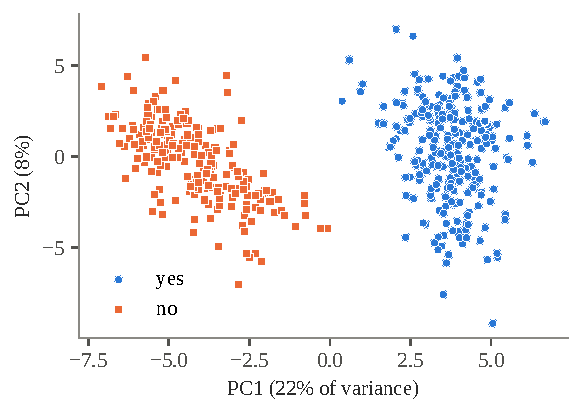
\includegraphics[width=0.5\textwidth]{fig3_pca.pdf}
\caption{All \NWords{} words on the first two principal components of the standardised features.}\label{fig:pca}
\end{figure}

\subsection{Noise}
Figure~\ref{fig:noise} and Table~\ref{tab:noise} show the noise results. With clean training, the models are still good at 20~dB but drop quickly after that. Naive Bayes is the best at 10~dB and then falls sharply. From 5~dB downwards logistic regression stays ahead, with \LRcleanZero\% at 0~dB. At the same level the SVM gives \SVMcleanZero\%, the MLP \MLPcleanZero\%, and the other models are also close to the \Major\% of the majority class. I expected the more flexible models to do better here, so this result surprised me. One possible reason is that a linear model depends less on the fine details of clean data, but I did not test this.

\begin{figure}[H]\centering
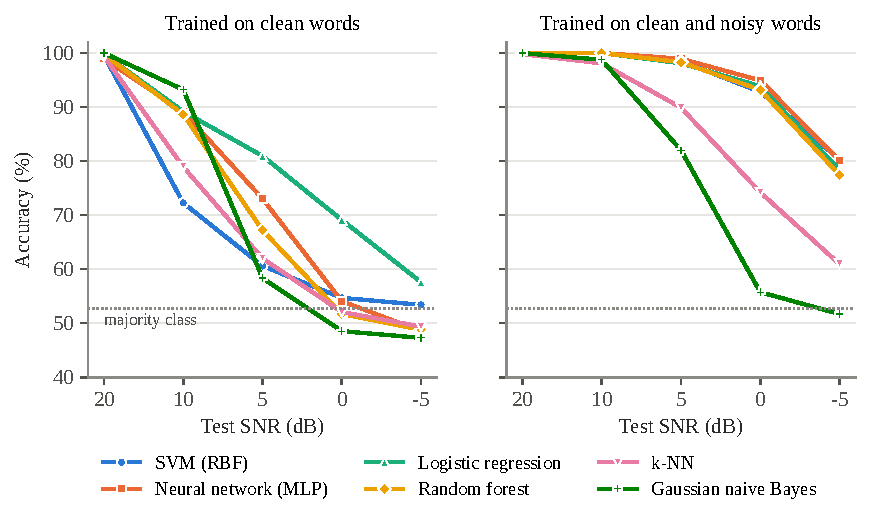
\includegraphics[width=0.92\textwidth]{fig4_noise.pdf}
\caption{Accuracy against test SNR. Both panels use the same vertical scale, and each point is the mean of 5 folds.}\label{fig:noise}
\end{figure}

Multi-condition training changes the picture far more than the choice of model does. At 0~dB the MLP reaches \MLPmultiZero\% and the SVM \SVMmultiZero\%, with logistic regression and the random forest in the same range. The standard deviation across folds is 1--3 points for these four, so I cannot say that one of them is better. k-NN and naive Bayes gain much less, with \KNNmultiZero\% and \NBmultiZero\% at 0~dB. Note that the noise levels from 20 to 0~dB and the noise type were all seen in training, so this is a favourable case. The only unseen level is $-5$~dB, where the four better models give about 77--80\% (SVM \SVMmultiMinus\%, MLP \MLPmultiMinus\%).

\begin{table}[H]\centering\small
\caption{Accuracy (\%) on noisy test words, mean $\pm$ std over 5 folds.}\label{tab:noise}
\setlength{\tabcolsep}{2.5pt}\footnotesize\begin{tabular}{lcccccc}\toprule
& \multicolumn{3}{c}{Trained on clean words} & \multicolumn{3}{c}{Trained on clean and noisy words}\\\cmidrule(lr){2-4}\cmidrule(lr){5-7}
Classifier & 10 dB & 5 dB & 0 dB & 10 dB & 5 dB & 0 dB\\\midrule
SVM (RBF) & 72.3 $\pm$ 9.4 & 60.6 $\pm$ 7.3 & 54.7 $\pm$ 1.5 & 100.0 $\pm$ 0.0 & 98.5 $\pm$ 1.2 & 92.8 $\pm$ 2.5\\
Neural network (MLP) & 89.1 $\pm$ 3.1 & 73.0 $\pm$ 7.9 & 54.1 $\pm$ 5.5 & 100.0 $\pm$ 0.0 & 98.9 $\pm$ 0.7 & 94.9 $\pm$ 1.3\\
Logistic regression & 89.2 $\pm$ 2.5 & 80.9 $\pm$ 4.1 & 69.1 $\pm$ 6.7 & 100.0 $\pm$ 0.0 & 98.1 $\pm$ 1.1 & 93.8 $\pm$ 2.3\\
Random forest & 88.6 $\pm$ 7.3 & 67.2 $\pm$ 10.0 & 51.7 $\pm$ 4.5 & 100.0 $\pm$ 0.0 & 98.3 $\pm$ 1.2 & 93.2 $\pm$ 2.2\\
k-NN & 78.9 $\pm$ 8.8 & 62.0 $\pm$ 10.0 & 52.1 $\pm$ 7.1 & 98.1 $\pm$ 1.6 & 89.9 $\pm$ 3.3 & 74.2 $\pm$ 3.9\\
Gaussian naive Bayes & 93.2 $\pm$ 7.3 & 58.4 $\pm$ 19.3 & 48.5 $\pm$ 3.3 & 98.8 $\pm$ 1.1 & 82.0 $\pm$ 4.6 & 55.7 $\pm$ 3.7\\
\bottomrule\end{tabular}\end{table}


\subsection{Amount of training data}
Figure~\ref{fig:lc} shows how little data this task needs. With one recording, which means eight words, k-NN reaches \KNNlcOne\% and the MLP \MLPlcOne\%. All models pass 99\% with five recordings. The SVM starts lowest, with \SVMlcOne\% on one recording, \SVMlcThree\% on three and \SVMlcFive\% on five. Its settings ($C=1$, $\gamma=0.001$) were mostly chosen on about 47 recordings, and they are probably too strongly regularised for a few words, so I do not read this curve as a general weakness of the SVM. Since these settings were chosen on recordings that can also appear in this test, the curve is a rough guide and not a strict evaluation.

\begin{figure}[H]\centering
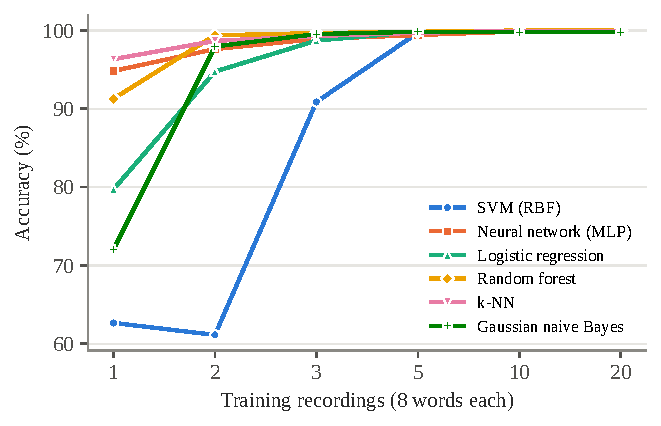
\includegraphics[width=0.56\textwidth]{fig5_learning_curve.pdf}
\caption{Accuracy on 15 held-out recordings against training size, averaged over 20 random draws.}\label{fig:lc}
\end{figure}

\subsection{Computation time}
Table~\ref{tab:cost} shows that time is not a problem for any model. The slowest at prediction, the random forest, takes about 0.1~ms per word, and fitting takes less than two seconds even with the grid search. These times come from one machine and will change on another one.

\begin{table}[H]\centering\small
\caption{Average cost per training fold and per word on the 2-core machine used here. Fit time includes the grid search, and naive Bayes has no grid, so its figure is not directly comparable.}\label{tab:cost}
\begin{tabular}{lcc}\toprule Classifier & Fit with tuning (s) & Prediction (ms/word)\\\midrule
SVM (RBF) & 0.10 & 0.014\\
Neural network (MLP) & 0.89 & 0.007\\
Logistic regression & 0.06 & 0.006\\
Random forest & 1.71 & 0.103\\
k-NN & 0.05 & 0.012\\
Gaussian naive Bayes & 0.00 & 0.006\\
\bottomrule\end{tabular}\end{table}


\subsection{Filter bank energies against MFCCs}
Since MFCCs are only a DCT of the log filter bank energies, I wanted to see whether the DCT step helps here. I repeated the experiments with the 26 log energies, using the same statistics and deltas (156 values), the same splits and the same noise. In each word I subtracted one overall mean as a level correction. Table~\ref{tab:fbank} compares the two features.

\begin{table}[H]\centering\small
\caption{Accuracy (\%) with 26 log filter bank energies (FB) and with MFCCs, on the same splits and the same noise.}\label{tab:fbank}
\setlength{\tabcolsep}{4pt}\begin{tabular}{lcccccc}\toprule
& \multicolumn{2}{c}{Clean words} & \multicolumn{2}{c}{10 dB, clean training} & \multicolumn{2}{c}{0 dB, multi-condition}\\\cmidrule(lr){2-3}\cmidrule(lr){4-5}\cmidrule(lr){6-7}
Classifier & FB & MFCC & FB & MFCC & FB & MFCC\\\midrule
SVM (RBF) & 99.66 & 99.79 & 52.7 & 72.3 & 90.5 & 92.8\\
Neural network (MLP) & 99.62 & 100.00 & 52.7 & 89.1 & 90.3 & 94.9\\
Logistic regression & 100.00 & 100.00 & 52.7 & 89.2 & 88.4 & 93.8\\
Random forest & 100.00 & 100.00 & 67.8 & 88.6 & 91.4 & 93.2\\
k-NN & 99.66 & 99.75 & 60.4 & 78.9 & 62.6 & 74.2\\
Gaussian naive Bayes & 99.79 & 99.79 & 74.5 & 93.2 & 47.9 & 55.7\\
\bottomrule\end{tabular}\end{table}


On clean words there is again almost no difference. With clean training, MFCCs are clearly better at 10~dB for all six models. At 0~dB the random forest and naive Bayes actually score higher with filter bank energies (59\% and 58\%), but both are still poor. With filter bank energies, the SVM, the MLP and logistic regression all give exactly the majority rate of \Major\% at 10, 5 and 0~dB. I checked one fold and found that they label every noisy word as ``yes'', so even mild noise moves the whole set across their decision boundary. My guess is that white noise lifts the weak bands together, and the correlated energies carry this shift straight into the model, but I did not test this. Multi-condition training removes most of the problem, although MFCCs stay about 2--5 points ahead at 0~dB for the four better models, and part of this gap is within the spread across folds.

\section{Discussion}
On clean words I cannot say that one classifier is better, because all of them almost reach the ceiling. The noise experiment gave me two more useful results. Training on noisy data helped much more than changing the classifier, and the most flexible models were not the most robust when they had only seen clean words. If I had to choose one model for this data, I would use logistic regression or the MLP with multi-condition training. Their results cannot be separated here, so I would prefer logistic regression because it is simpler.

Both of my feature sets depend on a hand-designed filter bank. wav2vec 2.0~\cite{wav2vec} takes a different route and learns its features from the raw waveform with a CNN encoder. During pre-training it hides about 49\% of the encoded time steps, which is similar to masked language modelling in BERT, where hidden words are predicted from their context~\cite{mlm}. A Transformer then has to pick the true quantised vector for each masked step from a set that also holds 100 distractors. After this, little labelled data is needed: with ten minutes of labelled speech the paper reports a WER of 4.8/8.2 on the clean/other test sets. My learning curve shows that labels are not the difficulty on this corpus, so the gain from such a model would show on a harder task with many speakers. I did not try it here. It would need a pre-trained model and 16~kHz audio, while this corpus is at 8~kHz.

These results have clear limits:
\begin{itemize}[nosep,leftmargin=*]
\item All recordings come from one speaker, so nothing here tells us how the models would work on another voice.
\item The task has only two short words, which is very far from real speech recognition.
\item The noise is white noise added after segmentation. In a real noisy recording the energy-based segmentation would probably fail before the classifier does, and this is one reason a proper VAD matters.
\item Each SNR uses a single noise realisation and only 5 folds, so small differences mean very little.
\item I used a small MLP on summary features and did not try a CNN on spectrograms, since the clean task leaves little room for improvement.
\end{itemize}

\section{Conclusion}
I segmented the Yes/No recordings into words, described each word with MFCC statistics, and compared six classifiers using splits made per recording. All six reached at least 99.7\% on clean words, compared with \TimeBase\% for the simple time-domain values. Noise gave a better comparison: at 0~dB most models trained on clean words were close to chance, while multi-condition training brought the SVM, MLP, logistic regression and random forest above 92\%. Removing the DCT did not matter on clean words, but MFCCs were more stable under noise. The main thing I learned is that a very high score on an easy data set says little about a model, and that how we split the data and what we train on can matter more than the classifier. The next step would be a data set with many speakers, such as Google Speech Commands, using pre-trained wav2vec 2.0 features as well as MFCCs.

\begingroup\small
\begin{thebibliography}{9}\setlength{\itemsep}{0pt}
\bibitem{openslr} ``Yes/No,'' Open Speech and Language Resources, SLR1. \url{https://www.openslr.org/1/}
\bibitem{khalooei} M. Khalooei, ``Kaldi Speech Recognition Toolkit Tutorial.'' \url{https://github.com/khalooei/kaldi-tutorial}
\bibitem{davis} S. Davis and P. Mermelstein, ``Comparison of parametric representations for monosyllabic word recognition in continuously spoken sentences,'' \emph{IEEE Trans. Acoustics, Speech, and Signal Processing}, vol. 28, no. 4, pp. 357--366, 1980.
\bibitem{cortes} C. Cortes and V. Vapnik, ``Support-vector networks,'' \emph{Machine Learning}, vol. 20, no. 3, pp. 273--297, 1995.
\bibitem{sklearn} F. Pedregosa et al., ``Scikit-learn: Machine learning in Python,'' \emph{Journal of Machine Learning Research}, vol. 12, pp. 2825--2830, 2011.
\bibitem{filterbank} ``Filter bank,'' Wikipedia. \url{https://en.wikipedia.org/wiki/Filter_bank}
\bibitem{wav2vec} A. Baevski, H. Zhou, A. Mohamed and M. Auli, ``wav2vec 2.0: A framework for self-supervised learning of speech representations,'' arXiv:2006.11477, 2020.
\bibitem{mlm} ``Masked language model,'' Coursera Articles. \url{https://www.coursera.org/articles/masked-language-model}
\end{thebibliography}
\endgroup
\end{document}
